%------------------------------------------------------------
%	CAPITULO I
%------------------------------------------------------------

\chapter{Diseño de interfaces de usuario basadas en voz}
\label{capIII}

% REFERENCIA
Dix, Finlay, Abowd y Beale (2004), señalan que la interacción entre humano y computadora, es la forma en que un usuario se comunica y se relaciona con un sistema computacional, así como la forma en que un usuario utiliza una computadora como herramienta para resolver o facilitar distintas tareas.

La comunicación entre un usuario y un sistema se logra gracias a un intermediario llamado interfaz. Esta se encarga de realizar las traducciones necesarias para hacer posible la comunicación de una manera más clara e idealmente efectiva, fácil, eficiente y agradable, con el fin de realizar el mejor proceso de comunicación posible. Sin embargo, la interfaz puede fallar al comunicar cierta información, por lo que la comunicación podría ser errónea, confusa y difícil. Es por ello que surgen distintos modelos de interacción, que permiten entender lo que sucede durante la interacción con un sistema y la identificación del posible origen de las dificultades.

Uno de los modelos de interacción más sobresalientes se conoce como el Modelo de Normal, basado en el ciclo de ejecución-evaluación de Norman. Este modelo se forma de dos componentes: la ejecución de tareas por parte de la computadora; y la evaluación por parte de los usuarios. Cuando un usuario manifiesta un plan y lo comunica por medio de una interfaz a la computadora, esta se encarga de ejecutar las acciones necesarias para dar una respuesta, misma que se transmite por la interfaz, para finalmente ser evaluada por el usuario. La ejecución  y evaluación involucradas en el proceso de comunicación del Modelo de Norman, se divide en siete fases que se presentan a continuación.

\begin{enumerate}
  \item Establecer el objetivo
  \item Crear la intención
  \item Especificar la secuencia de la acción
  \item Ejecutar la acción
  \item Percibir el estado del sistema
  \item Interpretar el estado del sistema
  \item Evaluar el estado del sistema, dependiendo de los objetivos y las acciones
\end{enumerate}

En las primeras fases, el usuario debe establecer un objetivo sobre aquellas tareas que requiere lograr o satisfacer, mismas que después debe traducir y adaptar para comunicar al sistema. Esta traducción se convierte en una secuencia de acciones que posteriormente se ejecutan en el sistema, lo cual provoca un cambio en el estado del sistema con la respuesta de la solicitud realizada. Estos resultados son interpretados y evaluados por el usuario, tomando en cuenta los objetivos y acciones definidas. Si la evaluación arroja resultados favorables y refleja los objetivos, entonces la interacción entre el usuario y el sistema se considera como exitosa. De lo contrario, el usuario genera un nuevo objetivo y repite todos los pasos, es por ello que el modelo se considera como un ciclo de ejecución y evaluación.

Para ilustrar el proceso descrito anteriormente, supongamos que una persona se encuentra viendo una película y decide comer palomitas de maíz, convirtiéndo esto en un objetivo. La intención se crea en forma de poner palomitas de maíz en el microondas. La secuencia de la acción puede ser el hecho de levantarse, colocar las palomitas en el microondas y establecer un tiempo adecuado para la preparación. En caso de que haya alguien cerca del microondas la intención y la secuencia de acción puede modificarse, si la intención se convierte en pedir a alguien que prepare las palomitas. En este ejemplo, el objetivo es el mismo, pero la intención y las acciones pueden variar. Cuando se ejecuta la acción y las palomitas están preparadas, se percibe el cambio de estado con el resultado. A este resultado se le interpreta y evalúa dependiendo de la percepción, es decir, si las palomitas están bien preparadas, entonces el ciclo se ha completado, de lo contrario, se genera un nuevo objetivo dependiendo del resultado, por ejemplo, si las palomitas se quemaron el nuevo objetivo es preparar unas palomitas nuevas, pero si a las palomitas les faltó más tiempo en el microondas, el nuevo objetivo es llevarlas nuevamente al microondas.

Es importante mencionar que durante el proceso pueden surgir eventos inesperados o excepcionales que se dividen en dos categorías: resbalones (slips) y equivocaciones (mistakes). Si el usuario conoce el comportamiento del sistema, así como las respuestas esperadas a las solicitudes y accidentalmente presiona algún botón o ejecuta alguna acción no planeada, entonces se considera como un resbalón. Por otro lado, si el usuario no conoce el sistema por completo y ejecuta alguna acción, recibiendo una respuesta que no esperaba, entonces se considera una equivocación.

Este modelo permite entender de forma más clara e intuitiva la interacción del usuario con el sistema, sin embargo, no detalla la interacción del sistema con el usuario por medio de la interfaz. Existe una extensión del Modelo de Norman, propuesto por Abowd y Beale, que se enfoca en la interacción del sistema por medio de la interfaz. 

La extensión del modelo de Norman para la interacción del sistema con el usuario se divide en cuatro componentes: el sistema, el usuario, las entradas y las salidas. El ciclo asociado a este modelo se compone de cuatro pasos que se muestran a continuación.

\begin{itemize}
  \item Articulación
  \item Rendimiento
  \item Presentación
  \item Observación
\end{itemize}

Los componentes, así como los pasos de transición entre componentes se muestra en la figura \ref{fig:31}.

% \begin{figure}[h]
\begin{figure}
  \centering
  \includegraphics[width=0.70\textwidth]{Cap3/Figuras/Transacción entre componentes.jpg}
  \caption{Transición entre componentes del Modelo de Norman para sistemas (2004).}
  \label{fig:31}
\end{figure}

El ciclo comienza con el usuario, quien es el encargado de crear un objetivo y una tarea o secuencia de acciones para realizar alguna tarea con ayuda del sistema. La forma en que el usuario comunica al sistema la información necesaria para realizar la tarea se transmite a partir de la articulación. En este paso, el usuario comunica las entradas al sistema por medio de la articulación, pasando al componente de entradas. Estas entradas son llevadas al sistema por medio del rendimiento, el cuál es un proceso que se encarga de traducir las entradas en operaciones. El sistema se encarga de transmitir las operaciones y todos los datos abstractos en una forma que pueda ser entendida por el usuario por medio de la presentación. Finalmente, estas salidas son mostradas o dadas a conocer al usuario por medio de una interfaz, en donde el usuario puede consultar los resultados de la tarea por medio de la observación.

Tal como se mencionó anteriormente, esta extensión del Modelo de Norman está enfocado en la interacción del sistema con el usuario, es decir, analizar los posibles puntos de dificultad del sistema para el usuario. En el primer paso de este modelo, es importante que el usuario pueda comunicar sus objetivos al sistema por medio de una articulación que pueda entender el sistema. Supóngase que el objetivo de un usuario es seleccionar un estado de la república mexicana. Dependiendo del sistema, el usuario podría articular está información por medio de la escritura del estado, sin embargo, esto está vulnerable a muchas dificultades, ya que un estado se podría escribir en mayúsculas, minúsculas, una combinación de ambas, por sus siglas o incluso escribir un texto que no es un estado. Otra forma de articular el mismo objetivo del usuario sería con una lista que contiene todos los estados válidos. En este caso, el usuario puede seleccionar un estado en un lenguaje que puede ser entendido y controlado por el sistema, ya que está limitado por sí mismo. En este paso se puede determinar qué tan buena es la facilidad de articulación que brinda el sistema para poder comunicar las entradas para realizar diferentes tareas.

En el siguiente paso las entradas pasan al sistema por medio del rendimiento. Este paso se enfoca principalmente en el manejo de los estímulos del sistema como respuesta a una solicitud con entradas específicas. Es decir, se determina el alcance de respuesta del sistema con entradas determinadas por el usuario. Por ejemplo, cuando se requiere ingresar información importante en un asistente basado en voz, tal como números de cuenta, el alcance para el estado de ingreso de información por medio de voz no está disponible por cuestiones de seguridad. Por otro lado, el alcance de ingreso de información importante sí es alcanzado por medio de la aplicación asociada al asistente. En el paso de rendimiento se puede determinar cuales son las acciones que pueden o no ser alcanzadas en distintas circunstancias, lo cuál, está directamente ligado a la implementación del sistema. Para el ejemplo anterior, el esfuerzo extra para el usuario es un control de seguridad que provee el sistema y que puede verse afectado en costo de implementación.

El paso de presentación consiste en traducir y mostrar los resultados de la consulta y la interacción anterior con el sistema. La traducción mostrada debe ser traducida de tal forma que se pueda transmitir de forma clara y 	fácil al usuario a partir de las herramientas con las que cuenta la interfaz. Es un proceso en el que se acopla la traducción del sistema hacia el usuario a través de la interfaz. Si la interfaz cuenta con pantalla, la información se puede transmitir visualmente, de lo contrario, se tendría que transmitir de otra manera, tal como información táctil o auditiva. Por otra parte, en este paso también se evalúa si la cantidad de información, así como la forma en que se presenta, es la más adecuada para facilitar la comunicación con el usuario. Finalmente, el usuario interpreta y evalúa la respuesta del sistema, donde se pueden tomar en cuenta puntos importantes de la interacción con el sistema como la facilidad de comunicación y el entendimiento de la respuesta por parte del sistema.

%------------------------------------------------------------
%	Interfaces de usuario
%------------------------------------------------------------

\section{Interfaces de usuario}
\label{InterfacesUsuarioCap3}

En términos tecnológicos, una interfaz de usuario es un medio que permite la interacción de un sistema interactivo entre una computadora y un usuario. Una interfaz de usuario se vuelve entonces, un intermediario entre la comunicación de mensajes de un sistema y una persona.

Una interfaz de usuario tiene como objetivo facilitar las necesidades o la realización de alguna tarea o acción específica, por lo que la comunicación entre el sistema y el usuario tiene que ser clara y fácil de entender. Esto se logra a partir de una interfaz usable, universal, sencilla de entender y que pueda generar resultados útiles.

% REFERENCIA
Shneiderman (2016) señala que los diseñadores de interfaces de usuario han desarrollado normas, a partir de la experiencia y práctica, para mejorar y lograr el diseño más adecuado de una buena interfaz de usuario. Estas normas se dividen en tres categorías, dependiendo de su nivel de importancia: guías, principios y teorías.

\begin{itemize}
  \item \textbf{Guías}: son consejos de bajo nivel sobre las buenas prácticas y precaución de peligros al momento de diseñar una interfaz de usuario.
  \item \textbf{Principios}: son estrategias o reglas de medio nivel, que permiten analizar y comparar las alternativas de diseño de la interfaz de usuario.
  \item \textbf{Teorías}: son marcos de alto nivel, que son fuertemente aplicables durante la etapa de diseño y evaluación de la interfaz de usuario. Por otra parte, estos marcos también apoyan el diseño de la comunicación y enseñanza del sistema para su mejor manejo.
\end{itemize}

% REFERENCIA
Un documento de guía, el cual proporciona consejos sobre las buenas prácticas, ayuda durante el proceso de desarrollo, proporcionando un mecanismo en el que se define el lenguaje y la terminología usada en un sistema. Shneiderman (2016) señala que los documentos de guía, promueven la consistencia en el diseño, apariencia y la secuencia de acciones. Así mismo, estos documentos almacenan las mejores prácticas de diseño derivadas de la experiencia y estudios empíricos, en los que se pueden incluir ejemplos y contraejemplos.

A continuación, se presentan algunos documentos de guía para diferentes aspectos de las interfaces de usuario.

\begin{itemize}
  \item \textbf{Navegación en la interfaz.} En ocasiones, la navegación en una interfaz de usuario puede ser complicada y confusa para algunos usuarios. El documento de guía presentado por el gobierno de Estados Unidos para el diseño de navegación en interfaces propone algunas recomendaciones como las siguientes:
  \begin{itemize}
    \item Estandarizar las secuencias para realizar tareas en un sistema.
    \item Asegurar que los mensajes mostrados sean descriptivos. 
    \item Utilizar encabezados descriptivos y únicos.
    \item Utilizar radio buttons para elecciones exclusivas.
  \end{itemize} 
  \item \textbf{Organización de elementos desplegados.} Un documento de guía enfocado a la organización de elementos de la interfaz, desarrollado por Smith y Moiser en 1986, ofrece cinco objetivos principales para presentar los datos o información en una interfaz, de tal forma que la organización sea la más adecuada y factible para el mejor control del sistema. Estos cinco objetivos se muestran a continuación:
  \begin{itemize}
    \item Consistencia de información presentada.
    \item Mostrar la información más adecuada y eficiente para el usuario.
    \item Presentar la cantidad mínima de datos.
    \item Compatibilidad entre la información mostrada con la información de entrada.
    \item Flexibilidad de recuperación de datos para el usuario.
  \end{itemize}
  \item \textbf{Obtención de atención del usuario.} El documento de guía llamado Wickens et al., creado en el año 2012, se enfoca en definir algunas guías para lograr obtener la atención del usuario. Algunos de estos consejos se muestran a continuación.
  \begin{itemize}
    \item Subrayar, encerrar, señalar con una flecha o utilizar cualquier forma de marcado para resaltar información relevante durante el proceso.
    \item Utilizar hasta cuatro diferentes tamaños para los elementos y usar el más grande para atrapar la atención del usuario.
    \item Elección de fuentes. Utilizar hasta tres diferentes tipos de fuentes.
    \item Utilizar tonos suaves para retroalimentación positiva y tonos más fuertes para condiciones de emergencia o error.
  \end{itemize}
  \item \textbf{Facilitar la entrada de datos o información de los usuarios.} Un ejemplo de documento de guía enfocado a la entrada de datos es el documento creado por Courtesy of MITRE Corporate Archives, en 1986. El cual propone algunos consejos como los que siguen:
  \begin{itemize}
    \item Consistencia en las transacciones de los datos de entrada.
    \item Mínima cantidad de acciones para la entrada de datos del usuario.
    \item Mínima cantidad de memoria cargada en el usuario.
    \item Compatibilidad de los datos de entrada con la información desplegada en la interfaz.
    \item Flexibilidad en el control de los datos de entrada.
  \end{itemize}
\end{itemize}

Como se muestra anteriormente, las guías se enfocan a cierto rubro de la interfaz y fungen como consejos para ser aplicados de forma limitada. Por otra parte, los principios tienen un enfoque más aplicable y duradero para el diseño de interfaces. Algunos principios están relacionados en los cinco estilos primarios de interacción, presentados a continuación.

\begin{itemize}
  \item \textbf{Manipulación directa.} Es la representación visual del mundo al momento de realizar una acción. Se busca simplificar las tareas con la representación de objetos familiares para el usuario.
  \item \textbf{Navegación y selección de menú.} Se determina una estructura clara para tomar decisiones para realizar las tareas definidas en el sistema. Asimismo, brindan una estrategia para garantizar un diseño consistente.
  \item \textbf{Llenado de formularios.} Este tipo de interacción está más enfocado a usuarios con más experiencia y conocimiento de los sistemas, ya que se debe tener conocimiento de los valores permitidos de entrada.
  \item \textbf{Lenguaje de comandos.} Brinda a los usuarios una sensación de control sobre el sistema, en la cual se aprende la sintaxis y se expresan posibilidades complejas sin la necesidad de instrucciones de uso.
  \item \textbf{Lenguaje natural.} Se implementan, por lo general, cuando las tareas requeridas por un usuario son diversas, tal como uso de contexto, sensores, gestos, comandos hablados, sonido, etc.
\end{itemize}

Los cinco estilos primarios de interacción tienen ventajas y desventajas, dependiendo del tipo de interfaz que se requiera diseñar. En particular, la ventaja que menciona Shneiderman sobre el estilo primario de interacción de lenguaje natural es que alivia la carga de aprendizaje de sintaxis del sistema. Por otro lado, una desventaja que menciona, es que requiere diálogos de aclaración detallados.

Además, existen unas reglas fundamentales que forman parte de los principios del diseño de interfaces de usuario, conocidas como \textit{Las ocho reglas de oro del diseño de interfaces}. Estas ocho reglas se presentan a continuación.

\begin{enumerate}
  \item \textbf{Esforzarse por la consistencia.} Deben definirse secuencias consistentes de acciones para situaciones similares.
  \item \textbf{Usabilidad universal.} Reconocer las necesidades de diversos usuarios, facilitando la transformación de contenido. Es decir, considerar la inclusión de funcionalidades para usuarios principiantes y expertos en el uso del sistema.
  \item \textbf{Mostrar comentarios informativos.} Dar retroalimentación para cada acción del usuario, en donde la respuesta sea modesta para acciones menores, mientras que para las acciones importantes, la respuesta debe ser sustancial y suficientemente detallada.
  \item \textbf{Diseñar diálogos para el cierre de acciones.} La secuencia de cualquier acción del sistema debe presentar un inicio, un punto medio y un final. Esto brinda una sensación de alivio, y satisfacción de logro para realizar las siguientes acciones.
  \item \textbf{Prevención de errores.} Implementar un sistema preventivo de errores para que el usuario no pueda cometer errores graves, y en caso de ocurrir, proveer instrucciones simples, constructivas y específicas para su recuperación.
  \item \textbf{Permitir un fácil retroceso de acciones.} Las acciones deben ser reversibles en lo posible, con el fin de aliviar la ansiedad de los errores que pudieran ocurrir. Esto brinda la posibilidad de deshacer acciones no esperadas por el usuario.
  \item \textbf{Mantener el control en los usuarios.} Cuando los usuarios ya conocen el manejo de una interfaz, no quieren cambios en el comportamiento que ya es familiar, por lo que se determina la familiaridad de las acciones de la interfaz si hay cambios en el diseño.
  \item \textbf{Reducir la carga de memoria a corto plazo.} El procesamiento de información en memoria a corto plazo de los seres humanos es limitado, por lo que es requerido que los usuarios eviten recordar información del sistema que usarán próximamente en otra parte del flujo del sistema.
\end{enumerate}

Finalmente, las teorías representan un marco con fundamentos fuertemente aplicables a las interfaces de usuario. Existen diferentes tipos de teorías que se presentan a continuación:

\begin{itemize}
  \item \textbf{Descriptivas.} Son útiles para desarrollar terminología consistente para un sistema.
  \item \textbf{Explicativas.} Describen la secuencia de eventos de un sistema, en el que se procura desarrollar la causa y efecto de las acciones.
  \item \textbf{Descriptivas.} Brindan una guía para tomar decisiones del diseño de forma más clara.
  \item \textbf{Predictivas.} Permite comparar los diseños propuestos, considerando el tiempo de ejecución, las tasas de error, o niveles de confianza.
\end{itemize}

Asimismo, algunas teorías también se enfocan en determinar una guía para la evaluación y el diseño de las interfaces de usuario. Estos se dividen en teorías micro-HCI y macro-HCI.

Las teorías micro-HCI se concentran en el rendimiento que puede ser medido en la interfaz, tal como la velocidad y los errores que pueden ocurrir en múltiples tareas. Entre estas teorías se encuentran las siguientes:

\begin{itemize}
  \item \textbf{Diseño por niveles.} Comienza con un diseño de alto nivel, que posteriormente se adapta a acciones más pequeñas.
  \item \textbf{Etapas de acción.} Considera el comportamiento del usuario a medida que manejan el sistema para lograr sus objetivos.
  \item \textbf{Consistencia.} Se considera la consistencia presentada en íconos, colores, formas, respuestas u opciones del sistema.
\end{itemize}

Por otro lado, las teorías macro-HCI se enfocan a casos resultantes de la experiencia del usuario durante semanas usando una interfaz de usuario, en las que se evalúan contextos reales. Estas teorías consideran los siguientes aspectos:

\begin{itemize}
  \item \textbf{Contextualizar.} Apoyar a los usuarios que se encuentran envueltos en un ambiente emocional, físico y social.
  \item \textbf{Dinámico.} Se enfoca al diseño para la evolución del comportamiento conforme el usuario avanza en los niveles del sistema.
\end{itemize}

%------------------------------------------------------------
%	Interfaces de usuario basadas en voz
%------------------------------------------------------------

\section{Interfaces de usuario basadas en voz}
\label{InterfacesUsuarioBasadasVozCap3}

%------------------------------------------------------------
%	Interacción basada en voz
%------------------------------------------------------------

\subsection{Interacción basada en voz}
\label{InteraccionBasadaVozCap3}

Existen cinco sentidos que puede percibir el ser humano: vista, oído, tacto, gusto y olfato, donde predomina el sentido de la vista al diseñar una interfaz de usuario, por lo que los sistemas utilizan elementos visuales como principal medio de presentación.

% REFERENCIA
Dix, Finlay, Abowd y Beale (2004), señalan que las interfaces de usuario basadas en voz son un tipo de interfaces inteligentes, también conocidas como interfaces multimodales, las cuales reciben este nombre por la combinación de diferentes canales de presentación basados en los cinco sentidos del ser humano. Es decir, las interfaces inteligentes o multimodales son un tipo de interfaces que permiten percibir y presentar información mediante estímulos visuales, auditivos, táctiles, gestuales, entre otros. Este tipo de interfaces tiene el objetivo de mejorar la interacción entre el sistema y el usuario, con el fin de facilitar la solución a un problema o una tarea.

Cada uno de los canales que pueden ser aplicados a una interfaz inteligente tienen la capacidad de transmitir diferentes percepciones al usuario. El canal auditivo, que se basa en el sonido, permite monitorear los eventos que rodean a un usuario, reaccionando a los ruidos o reproduciendo señales que cambien la atención del usuario. Este canal también permite tener un efecto emocional o más directo por medio de conversaciones auditivas o música, por lo que es capaz de alterar estados de ánimo, crear imágenes visuales y evocar escenas o atmósferas en la mente del usuario.

Por otro lado, el tacto permite representar la retroalimentación táctil que actualmente se aplica en algunas herramientas comunes que se pueden encontrar en automóviles, instrumentos musicales o cualquier herramienta que requiere una interacción con el tacto. Este sentido puede crear un vínculo estrecho entre los individuos con la gran información no verbal que recibe. Este sentido puede ser aprovechado en las interfaces de usuario que están relacionados a las simulaciones, tal como simular el manejo de un avión, simular tocar un instrumento, entre otros.

Los sentidos del gusto y el olfato permiten a un usuario apreciar información útil de la vida cotidiana, tal como verificar si los alimentos están en buen estado, detectar los primeros signos de peligro, entre muchos otros. Estos sentidos permiten al usuario obtener información de su entorno que pueden causar placer o desagrado.

El ambiente con el que interactúa un usuario es multisensorial, en donde cada sentido proporciona diferentes tipos de información del mundo. La interacción entre un usuario con el mundo que nos rodea mejora con diferentes percepciones multisensoriales, por lo que los sistemas interactivos que manejan más de un canal de percepción tienen la capacidad de brindar una interacción más nutrida, que permite ajustar un sistema de interacción más apropiado a las capacidades de los usuarios.

Las interfaces inteligentes, además de asemejar una interacción humano-computadora más natural, también generan sistemas redundantes, en donde se brinda la misma información por diferentes canales de percepción. La redundancia tiene como objetivo proporcionar una experiencia equivalente a todos los usuarios, sin importar su canal principal de interacción.

% REFERENCIA
En particular, una interfaz basada en voz, es un tipo de interfaz inteligente que apoya su interacción principalmente en el canal auditivo, tanto desde el usuario como de la interfaz. Dix, Finlay, Abowd y Beale (2004), señalan que las interfaces basadas en voz permiten el acceso a usuarios con discapacidades visuales, acceder a información en ambientes poco iluminados, así como hacer útil el funcionamiento de diferentes tipos de aplicaciones que no ocupan espacio en una pantalla para mostrar información.

%------------------------------------------------------------
%	Procesamiento de la voz
%------------------------------------------------------------

\subsection{Procesamiento de la voz}
\label{ProcesamientoVozCap3}

Además, los autores señalan que el sonido es una herramienta fundamental para mejorar los criterios de usabilidad. Señalan que existe evidencia experimental que muestran que la confirmación al presionar teclas o generar un click por medio de audio, reduce los errores en un sistema. Otra ventaja en la usabilidad está enfocado en la rama de videojuegos, ya que las pruebas experimentales muestran que los jugadores obtienen un menor puntaje cuando el sonido no está, a comparación de cuando el audio se encuentra presente. 

El sonido en una interfaz puede ser producido por ruidos, audios, música, discursos, entre otros. Existen dos tipos de sonidos en los que se dividen todas las categorías anteriores: sonidos de voz y no voz. El sonido de voz es aquel que es producido por la voz de un individuo y transmite información o mensajes por medio del sentido de habla, mientras que los sonidos de no voz son aquellos que son producidos por ruidos, melodías o todo aquello que no sea producido por el sentido del habla. Cabe mencionar que puede haber una combinación de los dos tipos de sonido mencionados, como podcast, canciones, discursos con música de fondo, etcétera.

El habla es uno de los sentidos fundamentales para comunicar información, que se desarrolla desde temprana edad al imitar el habla de todas las personas que nos rodean. El proceso de aprender a hablar es complejo y estructurado, por lo que generar la síntesis del habla por medio de una computadora se vuelve un desarrollo complicado. Por ejemplo, cuando se comienza a aprender un nuevo idioma, es fundamental conocer las reglas gramaticales, que proveen principalmente la estructura de cómo se componen las frases, con el fin de comunicarse con alguien que también conozca la estructura del habla. El diseño de comunicación por voz entre un usuario y un sistema es similar, en donde se debe $"$enseñar$"$ a la computadora a manejar las estructuras del lenguaje para poder comunicarse de la forma más natural posible.

Es primordial conocer la estructura del idioma en el que estará basada la interfaz, ya que con este conocimiento, se trata de lograr la mejor comunicación e interacción posible entre el usuario y el sistema de forma natural. Un posible conjunto de puntos importantes que son necesarios saber sobre el idioma, son los fonemas con los que se compone \footnote{Un fonema es la unidad mínima de sonido de un lenguaje hablado. Cada fonema representa un sonido distinto.}, el énfasis, el acento, las pautas, e incluso el tono en el que se transmite un mensaje para no modificar el significado de un enunciado. Al conocer la estructura del idioma (sintaxis) y la forma en que los puntos anteriores alteran su significado (semántica), es posible lograr la mejor forma de comunicación, donde se reconoce de mejor forma la recepción de mensajes del usuario y se comunica de forma correcta un mensaje de la interfaz al usuario.

Por otro lado, la percepción del sonido, que está relacionado al reconocimiento de voz por computadora, se vuelve complicada con problemas como la detección del ruido de fondo, ya que puede interferir al introducir sonidos que distorsionan el mensaje original. Otro problema es la introducción de pausas o muletillas como $"$ummm$"$, $"$este...$"$, $"$emmm$"$, etc, ya que el reconocimiento de voz podría detectar estos fragmentos de entrada como información útil para el sistema. Finalmente, otro problema que puede distorsionar la entrada, son los acentos tradicionales de cada región, ya que la variación del acento transforma las entradas del sistema de reconocimiento, ya que cada variación puede ser diferente con la forma en que se transmiten ciertos mensajes, así como el cambio de vocabulario.

Otro aspecto importante a considerar con el sonido producido por el habla, es la síntesis de la voz. Este aspecto se refiere al principio de poder tener una conversación natural con una computadora, en el que se refleje la interacción diaria entre dos personas. Uno de los retos más importantes para el reconocimiento de voz, es la sensibilidad a las variaciones y entonación del habla, por lo que la forma de transmitir información por medio de la interfaz debe ser clara y objetiva. Asimismo, la transmisión de voz de forma natural, desde la interfaz basada en voz, resulta difícil de adaptar con tonos monótonos y robotizados, en los que es muy probable notar la ausencia de sentimientos o entonación durante la emisión de mensajes. Para lograr una conversación natural entre una computadora y un usuario, es primordial conocer la forma de interacción del usuario, tomando en cuenta los puntos anteriores, así como el lenguaje, el vocabulario, modismos, frases e incluso la entonación o forma en que se transmiten los mensajes en una conversación cotidiana, con el fin de que el usuario pueda realizar sus tareas con el sistema, en un ambiente en el que se sienta identificado, satisfecho y cómodo.

Otro punto a considerar durante el diseño de las interfaces de usuario basadas en voz, está relacionado a la consulta y exploración del sistema. Al ser una interfaz cuyo canal principal es la voz, se vuelve complicado consultar información o acceder a la exploración general del sistema. En una interfaz visual, el usuario puede tener un panorama general de las tareas que puede realizar utilizando la interfaz, sin embargo, con la ausencia del sentido visual, las funcionalidades de la interfaz deben ser explicadas de forma sencilla y objetiva al usuario. Durante la realización de una actividad con un sistema basado en voz, es valioso tener un sistema de asistencia en el que se lleve paso a paso al usuario para lograr satisfactoriamente la finalización de la tarea. Para ello, durante el diseño de una interfaz basada en voz se debe considerar la división y las pautas que tomará cada actividad para no saturar de información al usuario y no olvide fácilmente el proceso tomado para realizar una tarea.

% REFERENCIA
Dix, Finlay, Abowd y Beale (2004), consideran otro tipo de voz hablada en una interfaz de usuario que no requiere el reconocimiento de voz para hacer funcionar la interacción de la interfaz, este tipo de voz hablada la denominan voz no interpretada. La cual consiste en mensajes pregrabados que son reproducidos en cada uno de los procesos con los que cuenta el sistema, con el fin de complementar o reemplazar información visual. Este tipo de voz hablada es generalmente usada en museos, con el propósito de que los espectadores comprendan de forma sencilla e interactiva el contenido de una sala. Este mecanismo es usado en interfaces que cuentan con un canal visual con el que puede interactuar el usuario para conocer información, y que al recibir retroalimentación de las funcionalidades, se retorna una salida visual y auditiva con la información pregrabada por voz. Al ser grabaciones hechas por una persona, por lo general tienen una entonación y pronunciación humana natural. Este sistema de grabaciones, puede resultar muy útil para interfaces especializadas para aplicaciones colaborativas o para anotaciones de audio que fungen como recordatorios, así como para sentir mayor empatía con la retroalimentación de un sistema al contar con una conversación más natural. Una de las aplicaciones más cotidianas se puede encontrar en las mesas de ayuda telefónica en compañías telefónicas, bancos o asistentes en tiendas virtuales dedicadas a la atención de clientes.

Los sonidos de voz dependen del idioma en que se requiera transmitir la información, por lo que se vuelve una labor complicada la extensión del funcionamiento de un sistema en diferentes idiomas. Los sonidos considerados como no voz, tienen ciertas ventajas que pueden enriquecer la forma de interacción entre los usuarios y una interfaz. Como estos sonidos no dependen de la voz, se puede aprovechar como respuesta en el uso de una adaptación auditiva, es decir, cada sonido del sistema estaría asociado a un significado específico. Por ejemplo, cuando una tarea está completa, se puede activar un sonido de afirmación o si ocurre un error, se puede producir un sonido de alerta. Sin embargo, la desventaja de los sonidos de no voz, es que el usuario debe estar familiarizado con estos y aprender el significado de cada uno de ellos, mientras que el significado del sonido por voz es claro y preciso porque está relacionado al lenguaje hablado.

% REFERENCIA
Algunas aplicaciones de los sonidos que no son por voz se pueden encontrar frecuentemente como indicaciones o cambios en el sistema, así como para denotar errores. Los sonidos sin voz también son útiles para proporcionar información relevante del manejo de un sistema a las interfaces se controlan con una navegación conocida como navegación auditiva. Dix, Finlay, Abowd y Beale (2004), señalan que los experimentos realizados con navegación auditiva demuestran que las pistas auditivas son adecuadas para que un usuario pueda diferenciar hasta ocho objetivos en una pantalla de forma rápida y con una precisión razonable, lo cual es efectivo para personas con discapacidades visuales.

Asimismo, el canal auditivo puede combinar el uso del sonido por voz y no voz, con el fin de crear un mejor medio de interacción de un usuario con la interfaz. Este se puede ejecutar como una respuesta con un fondo auditivo referente a la temática o respuesta dada por el sistema.

El proceso de información basada en voz con todas las herramientas mencionadas anteriormente puede mejorar el manejo de una interfaz de usuario, siendo un medio alternativo o principal. Este tipo de interfaces proporciona también un medio alternativo de entrada de información para usuarios con discapacidad visual, física o cognitiva. El canal auditivo se convierte además en un receptor que permite una menor esfuerzo de entrada para el usuario, ya que el habla es un canal de interacción que no requiere mucho esfuerzo a comparación de los canales visuales o táctiles.

%------------------------------------------------------------
%	Asistentes basados en voz
%------------------------------------------------------------

\subsection{Asistentes basados en voz}
\label{AsistentesBasadosVozCap3}

Con el considerable crecimiento del uso de teléfonos y celulares, las aplicaciones operadas con voz comenzaron a tener mayor popularidad. Estos dispositivos, que basan su funcionamiento en la voz han evolucionado a tal grado que hoy en día se cuenta con múltiples funcionalidades en un único dispositivo.

Actualmente existen dispositivos que permiten incluir el reconocimiento de voz en diferentes aplicaciones, tales dispositivos cuentan con un asistente virtual basado en voz, desarrollados con el propósito de mejorar la experiencia del usuario con herramientas mejoradas que son controladas por voz. Algunos de estos dispositivos se mencionan a continuación.

\begin{itemize}
  \item \textbf{Alexa}, desarrollado por la compañía \textit{Amazon.com, Inc}.
  \item \textbf{Google Home} y \textbf{Google Assistant}, desarrollados por la compañía \textit{Google}.
  \item \textbf{Siri}, perteneciente a la empresa \textit{Apple Inc}.
  \item \textbf{Cortana}, desarrollado por la empresa tecnológica \textit{Microsoft Corporation}.
  \item \textbf{Bixby}, desarrollado por \textit{Samsung}.
\end{itemize}

Estos dispositivos pueden realizar búsquedas para dar respuesta y resolver una tarea dada por un usuario, tal como responder alguna pregunta general, dar el clima, reproducir música, programar algún evento, entre muchos otros. En la figura \ref{fig:32}, se muestran los porcentajes de las peticiones de los dispositivos basados en voz por parte de los usuario, según la ComScore \footnote{Compañía de investigación de marketing en Internet que proporciona datos de marketing y servicios para muchas de las mayores empresas de Internet.}.

% \begin{figure}[h]
\begin{figure}
  \centering
  \includegraphics[width=0.70\textwidth]{Cap3/Figuras/Usos más frecuentes.png}
  \caption{Usos más frecuentes de los dispositivos basados en voz. Bratten, E. (2021).}
  \label{fig:32}
\end{figure}

Todas las peticiones mostradas, por lo general, requieren de una petición o una pregunta para activarse y poder funcionar, lo cual hace muy sencillo el funcionamiento de comunicación entre el dispositivo y el usuario, además de ser rápido al realizar una tarea. Sin embargo, un dispositivo basado en voz puede activarse sin necesidad de hacer una petición, por ejemplo, cuando se notifica una alarma o un recordatorio, lo cual mejora la experiencia de usuario al no estar al pendiente de una notificación visual o depender de la desactivación física de un dispositivo.

Esta última funcionalidad hacia los usuarios, abre la puerta a que el uso de dispositivos basados en voz aumente considerablemente y tenga mayor popularidad hoy en día. Por ejemplo, un usuario que está conduciendo un automóvil, podría realizar llamadas, tener control completo sobre la música en reproducción, saber la hora, conocer la dirección de un destino, escuchar podcast e incluso practicar un idioma o aprender recetas de cocina, todo, sin necesidad de tocar la pantalla de un dispositivo, lo cual provee al usuario, además de facilidad, seguridad a un usuario para no fijar la mirada en distractores como lo es una pantalla.

% REFERENCIA
De este ejemplo, se puede observar la gran ventaja de adaptar un dispositivo basado en voz mientras un usuario conduce. Pearl, C. (2016) menciona algunas otras ventajas más de usar este tipo de interfaces.

\begin{itemize}
  % REFERENCIA
  \item \textbf{Velocidad.} Incluso para los expertos en mensajes de texto, la facultad de hablar hace más rápido el proceso de comunicación. Un estudio de Stanford afirma que para comunicar información, el sentido del habla es más rápido que escribir. Shahani (2016) señala que esta afirmación está demostrada por un estudio realizado por  la Universidad de Stanford, la Universidad de Washington y Baidu.
  \item \textbf{Manos libres.} Tal como se mencionó en el ejemplo del conductor, realizar acciones como conducir o cocinar hace que hablar sea más práctico que escribir, además de proveer mayor seguridad al no generar distracciones al sentido de la vista.
  \item \textbf{Intuitividad.} Hablar es una habilidad muy bien desarrollada por la mayoría de la población, por lo que es muy intuitivo el manejo de una interfaz usando la voz como medio de comunicación.
  \item \textbf{Empatía.} La entonación de una frase dice mucho en cómo se comunica un mensaje. Es decir, no es lo mismo decir $"$estoy feliz$"$ en un tono alegre, emocionante y un tanto exaltado, a diferencia de decir exactamente la misma frase en un tono indiferente, triste y sin ánimo. La comunicación con un dispositivo basado en voz puede proveer más información que la que puede dar un dispositivo en texto o en imágenes.
\end{itemize}

% REREFENCIA
A pesar de las ventajas que pueden surgir con una interfaz basada en voz, es importante mencionar que no siempre es buena idea aplicarlas. A continuación se muestran algunos casos que propone Pearl (2016).

\begin{itemize}
  \item \textbf{Espacios públicos.} Es importante mantener privada cierta información, ya sea dada por el usuario o dada como respuesta desde el dispositivo. Si la información que está en juego entre la comunicación es de carácter privado o que los usuarios podrían considerar como privada o íntima, podría no ser buena idea usar una interfaz basada en voz, donde la información puede ser recibida por un tercero.
  \item \textbf{Incomodidad al hablar con una computadora.} A pesar de la facilidad de comunicación por voz, existen personas que no sienten comodidad al hablar con una computadora. Se vuelve un poco vergonzoso hablar $"$a la nada$"$. Si alguna aplicación está dirigida a usuarios que en su mayoría tienen esta dificultad, no es buena idea incluir el manejo por voz.
  \item \textbf{Usuarios que prefieren texto.} Cierto porcentaje de los usuarios prefieren usar un dispositivo por medio de texto porque sienten mayor facilidad del manejo en la interfaz.
  \item \textbf{Proteger la privacidad.} Relacionado un poco a la limitante de usar interfaces basadas en voz en lugares públicos, es importante proteger la privacidad de los usuarios. Esto es, no dar más información de la necesaria o información valiosa. Por ejemplo, si se quiere comprar algún producto por medio de voz, no se puede proporcionar el número de tarjeta ni claves por voz, ya que esto hace inseguro el sistema, ya que un tercero puede escuchar todos estos datos. No sólo por parte del usuario, sino también del sistema, por ejemplo, si este pide confirmación del número de cuenta repitiendo el número.
\end{itemize}

%------------------------------------------------------------
%	Diseño centrado en el usuario
%------------------------------------------------------------

\section{Diseño centrado en el usuario}
\label{DisenioCentradoUsuarioCap3}

La Asociación Profesional de Usabilidad o Usability Professionals Association (UPA), define el Diseño Centrado en el Usuario como un enfoque de diseño orientado a satisfacer las necesidades de los usuarios que harán uso de un producto o servicio.

% REFERENCIA
Hassan y Ortega (2009) señalan que los diseñadores consideraban que la optimización y adaptación de productos al ser humano  se origina de un proceso a un proceso de investigación, en particular en las áreas de antropometría, ergonomía, arquitectura o biomecánica, en el origen del diseño centrado en el usuario en la década de los cincuentas con el diseño industrial y militar.

A partir de está visión, varios diseñadores de la época comenzaron a utilizar la visión del diseño centrado en el usuario como una oportunidad para generar soluciones innovadoras para diferentes productos, que posteriormente se adaptaron tecnológicamente. Esto abrió un gran panorama para mejorar la funcionalidad en el diseño de diferentes productos que ofrecían nuevas y mejores métodos de trabajo para solucionar problemas.

% REFERENCIA
Hassan y Ortega (2009) mencionan que en la década de los ochenta se vuelve popular el diseño centrado en el usuario gracias a Norman, D., ya que comenzó a utilizar el término $"$User System Design$"$ (Diseño del Sistema de Usuario) en diferentes conferencias presentadas por su equipo en la CHI Conference (1983).

% REFERENCIA
El diseño centrado en el usuario comienza a partir de la observación de cómo los usuarios utilizan diferentes sistemas y a partir de ello crear modelos de los procesos de interacción. Hassan y Ortega (2009) señalan que se utilizaban tres términos que debían ser considerados para entender el proceso de observación para el análisis del diseño centrado en el usuario. Estos términos se presentan a continuación.

\begin{itemize}
  \item \textbf{Modelo conceptual.} Es toda la información que ofrece el diseñador del sistema.
  \item \textbf{Interfaz.} Se refiere al canal visual que ofrece el sistema al usuario.
  \item \textbf{Modelo mental.} Es la información que desarrolla el usuario a partir de la presentación en la interfaz.
\end{itemize}

Es así como el enfoque del diseño centrado en el usuario busca la funcionalidad adecuada para un conjunto de usuarios específicos. Con lo que se procura responder a preguntas como ¿quién usará este sistema?, ¿qué es lo que va a hacer con él? ó ¿qué información necesitará para alcanzar sus objetivos?, entre otras.

% REFERENCIA
Sin embargo, el diseño centrado en el usuario crea diferentes enfoques dependiendo de la filosofía de diferentes áreas. Kalbach (2007) menciona algunos enfoques que se presentan a continuación.

\begin{itemize}
  \item \textbf{Diseño centrado en el diseñador.} En este enfoque, se propone que el diseñador sabe qué es lo mejor para los usuarios, dependiendo de su visión.
  \item \textbf{Diseño centrado en la empresa.} El producto que se diseña debe satisfacer las necesidades de la empresa siguiendo una estructura definida.
  \item \textbf{Diseño centrado en el contenido.} En este enfoque la información provee una base para poder organizar la estructura de navegación del producto.
  \item \textbf{Diseño centrado en la tecnología.} Se busca la forma más sencilla de implementar la solución a los problemas que se presenten en el producto.
\end{itemize}

% REFERENCIA
Concretamente, Hassan y Ortega (2009) definen el diseño centrado en el usuario como un proceso cíclico en el que se toman decisiones de diseño se orientan al usuarios y los problemas que requiere solucionar con un sistema. Este proceso evalúa el diseño de la usabilidad iterativamente, con el fin de mejorar la interfaz o el sistema de forma incremental.

La norma ISO 13407 propone que el proceso iterativo del diseño centrado en el usuario se puede dividir en cuatro fases:

\begin{itemize}
  \item \textbf{Especificar el contexto de uso.} Se analiza e identifica a los usuarios que manejarán el producto final, así como reconocer el propósito y las condiciones en que será utilizado.
  \item \textbf{Especificar los requisitos.} Se identifican las necesidades del usuario, así como lo que se requiere proveer desde el sistema para satisfacer el objetivo o los objetivos.
  \item \textbf{Producir soluciones de diseño.} Se presentan soluciones conceptuales hasta crear una solución final para el diseño. Es importante mencionar que está fase puede subdividirse en diferentes fases.
  \item \textbf{Evaluación.} En está etapa se validan las soluciones de diseño, así como detectar problemas de usabilidad. Está etapa por lo general se realiza con usuarios que usarían el sistema a partir de un test.
\end{itemize}

El proceso iterativo para el diseño centrado en el usuario se lleva a cabo como en la figura \ref{fig:33}.

% \begin{figure}[h]
\begin{figure}
  \centering
  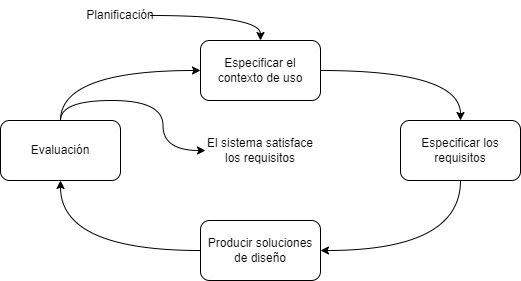
\includegraphics[width=0.70\textwidth]{Cap3/Figuras/DCU.jpg}
  \caption{Proceso del Diseño Centrado en el Usuario. Bratten, Concretamente, Hassan y Ortega (2009).}
  \label{fig:33}
\end{figure}

Es importante mencionar que este proceso también sugiere un enfoque para resolver problemas estratégicamente para mejorar su utilidad, es decir, durante el proceso se analiza la capacidad del producto para resolver necesidades.

Para lograr recabar toda la información necesaria para conocer al usuario, así como detectar sus necesidades, es a partir de la observación, investigación y análisis del usuario, tal como sus actividades, el entorno que percibe y el contexto en el que tomaría lugar el uso del producto.

% REFERENCIA
Para lograr los resultados más adecuados para el diseño centrado en el usuario, se recurre a guías que se denominan metodologías para el diseño centrado en el usuario. Bratten, Concretamente, Hassan y Ortega (2009), señalan que estás metodologías o técnicas tienen como objetivo conocer y comprender las necesidades de los usuarios, así como el comportamiento y limitaciones en casos reales en los que se usaría el sistema a partir de una interfaz. Con ello se pretende responder preguntas que ayudan a mejorar el diseño centrado en el usuario, tal que permitan determinar descripciones, procedimientos, ubicaciones, limitaciones y problemas que se pudieran presentar.

Para conocer cada una de las características y puntos mencionados anteriormente, se recurre a la aplicación de test o pruebas de un sistema a usuarios. Es importante tener en cuenta que estas pruebas pretenden evaluar el sistema y la usabilidad del diseño, más no al usuario.

%------------------------------------------------------------
%	Técnicas del análisis del usuario
%------------------------------------------------------------

\section{Técnicas del análisis del usuario}
\label{TecnicasAnalisisCap3}

Las técnicas del análisis del usuario permiten formar herramientas que proveen información específica y relevante de diferentes aspectos de los usuarios a los que va dirigido un producto. Está información puede incluir desde sus intereses personales, dificultades o frustraciones, emociones al usar un sistema o incluso identificar problemas que pueden ser atacados para facilitar la resolución de problemas en el sistema, producto o servicio desarrollado.

A continuación se describen dos técnicas del análisis del usuario, que permiten extraer información específica que es útil para el diseño del producto: Persona y Customer Journey Map.

%------------------------------------------------------------
%	Persona
%------------------------------------------------------------

\subsection{Persona}
\label{PersonaCap3}

La fundación de diseño de interacción, señala que la técnica conocida como Personas, consiste en crear personajes ficticios que cumplan con las características necesarias de los usuarios que podrían usar un producto o un servicio. Esta herramienta permite entender de mejor forma las necesidades, experiencias y comportamientos de los usuarios, lo cual provee información para mejorar el diseño de los productos.

Las herramientas resultantes de la técnica Personas, aportan un esquema de apoyo para el diseño de la experiencia de usuario, el cual genera empatía y acercamiento al mundo de los usuarios a través del producto diseñado. El objetivo principal de la técnica es definir de forma clara las necesidades identificadas en los usuarios, con el fin de establecer funcionalidades necesarias para implementar y aplicar en el producto final.

La fundación de diseño de interacción propone una serie de reglas para crear y diseñar de forma correcta un producto Persona que cumpla con su función adecuadamente. Estas reglas se mencionan a continuación:

\begin{enumerate}
  \item Recopilar la mayor cantidad de datos sobre los usuarios objetivos.
  \item Determinar las características que se comparten y difieren entre los usuarios.
  \item Desarrollar hipótesis resultantes de la investigación, considerando las cualidades y diferencias determinadas en el punto anterior.
  \item Confirmar que las partes interesadas estén de acuerdo con las hipótesis definidas en el punto anterior.
  \item Determinar la cantidad de personas involucradas para la creación del esquema Persona. Es importante concentrarse sólo en una persona para desarrollar el esquema.
  \item Nombrar y describir a cada persona en un esquema de una o dos páginas. Este apartado debe incluir la siguiente información.
  \begin{enumerate}[a)]
    \item Fotografía del usuario.
    \item Valores, intereses, educación, estilo de vida, necesidades, actitudes, deseos, limitaciones, metas y patrones de comportamiento del usuario.
    \item Detalles adicionales que hagan más real los datos del esquema, con el fin de generar más empatía.
  \end{enumerate}
  \item Describir situaciones en las que el usuario podría usar el producto y colocarlo en contextos con problemas a superar.
  \item Incluir a todos los involucrados del proyecto para aceptar a la persona o aconsejar revisiones.
  \item Enviar los datos recopilados para usar en el producto.
  \item Desarrollar los escenarios en los que se podría usar el producto. Estos deben exponer de manera clara a la persona en los posibles casos de uso.
  \item Realizar ajustes continuos para agregar nuevas características o descartar personas obsoletas.
\end{enumerate}

Una vez que las personas involucradas en el proyecto entienden de forma más clara a los usuarios, es pertinente definir el límite de los detalles a considerar para aportar a un producto, con el fin de delimitar aquellas características que se ajusten a los diseños. La fundación de diseño de interacción señala que con está información también se puede crear un prototipo con la recopilación de los datos más importantes, el cual debe incluir los siguientes puntos.

\begin{enumerate}
  \item Las características del usuario deben permanecer en contexto.
  \item Refleja de forma general el comportamiento, las actitudes, un conjunto de habilidades y motivaciones, así como los objetivos que tiene el usuario dentro del dominio del producto.
  \item Conocer el objetivo del usuario, lo que quiere resolver y los problemas que quiere abordar, así como las características que le ayudarían a resolver los problemas de mejor forma a como lo hace.
  \item Identificar e incluir los escenarios realistas que enfrenta el usuario, e imaginar cómo usarían el producto para lograr un objetivo particular.
  \item Ocupar un entorno coronado que muestre una rutina cotidiana del usuario.
  \item Identificar los aspectos de dificultar o frustración del usuario.
\end{enumerate}

A continuación se presenta un esquema final en la figura \ref{fig:34}, resultado de todos los puntos y aspectos mencionados anteriormente. En el siguiente ejemplo, se tiene una aplicación que permite buscar, controlar y reproducir música, la cual tiene el usuario llamado Rebecca, que representa a usuarios de 26 años que usan algunas aplicaciones como Spotify para reproducir música. A través del usuario Rebecca, se puede observar como la aplicación ayuda a usuarios con el mismo perfil o similar en su día a día. Imaginemos que Rebecca gusta de escuchar música de calidad, compartir música con amigos, familiares y tiene un mecanismo de clasificación de música de diferentes géneros. Su objetivo es reproducir música de calidad de forma rápida, cómoda y fácil.

% \begin{figure}[h]
\begin{figure}
  \centering
  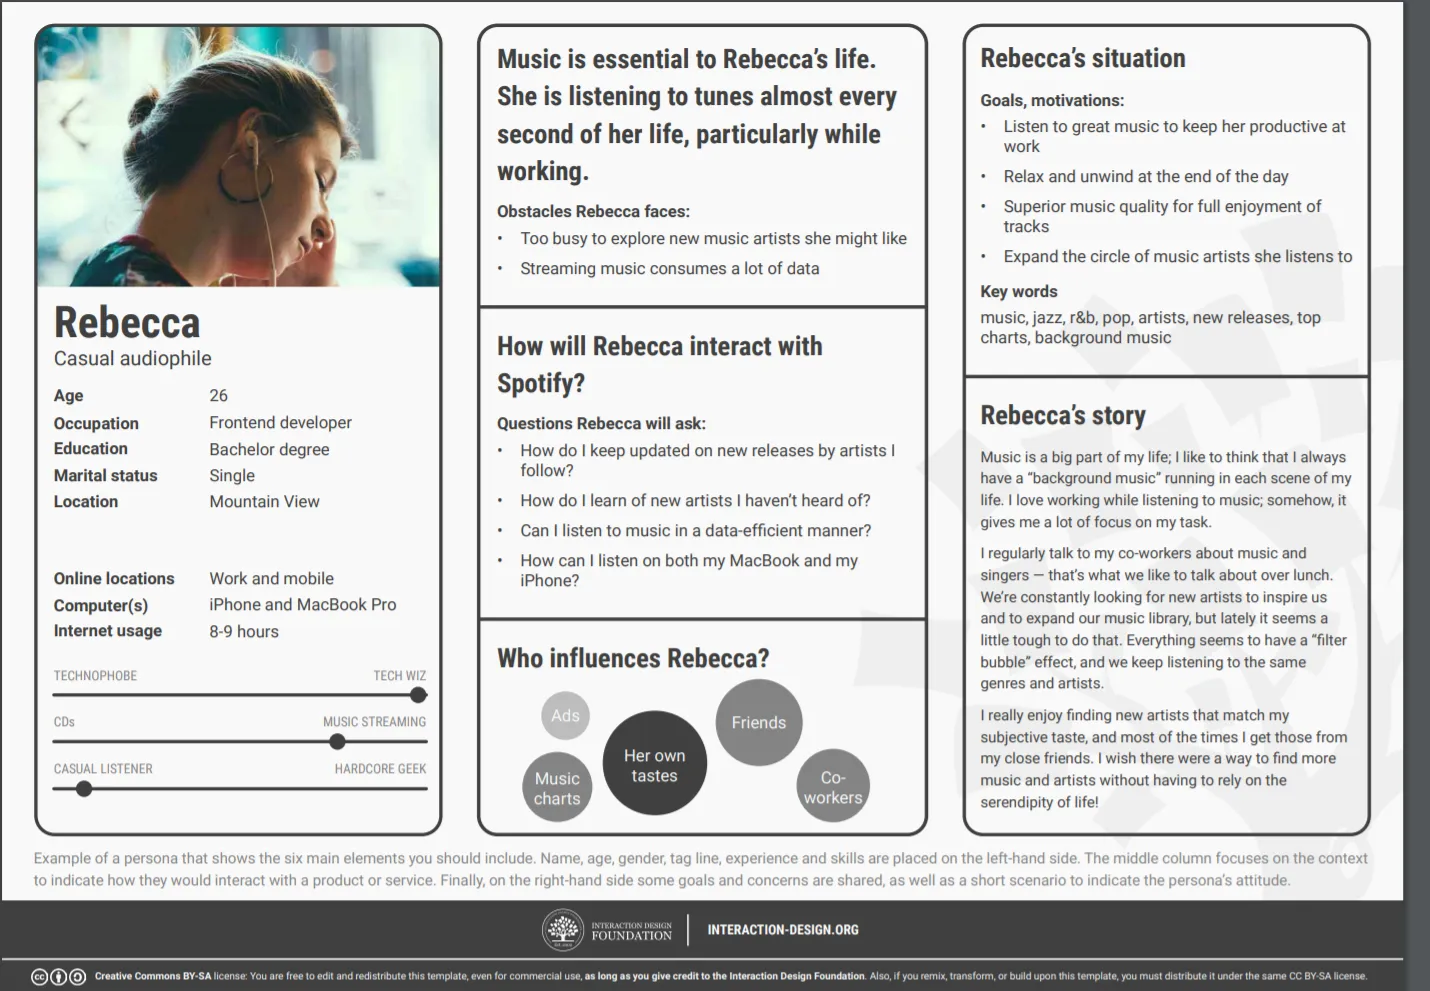
\includegraphics[width=0.70\textwidth]{Cap3/Figuras/EjemploPersona.jpg}
  \caption{Ejemplo de Persona. Interaction Design Foundation (2022a).}
  \label{fig:34}
\end{figure}

%------------------------------------------------------------
%	Customer Journey Map
%------------------------------------------------------------

\subsection{Customer Journey Map}
\label{CustomerJourneyMapCap3}

% REFERENCIA
Komninos y Briggs (2022) señalan que un Customer Journey Map es una herramienta que examina la historia de cómo un usuario se relaciona con un producto o servicio a lo largo del tiempo. Está herramienta sirve para generalizar una idea del viaje que podría tomar un usuario con un producto, lo cual proporciona información sobre las interacciones en cada punto de un sistema, así como la capacidad de mejora en la interacción del sistema con un usuario en iteraciones futuras.

Por otro lado, ayudan a facilitar la comprensión de cómo se debe tratar de forma general a los usuarios en diferentes contextos y puntos del sistema para realizar una tarea. Además permite determinar una organización detallada de cómo los usuarios progresan en el uso del producto para lograr sus objetivos o resolver subtareas, con el fin de determinar un proceso de comunicación amplio y centrado en el usuario.

Un Customer Journey Map también provee información sobre los sentimientos que siente un usuario en cada una de las etapas del uso de un producto. Permite explorar lo que los usuarios sienten, ven, oyen, hacen, plantean y piensan.

% REFERENCIA
Komninos y Briggs (2022) recomiendan preparar ciertos requisitos antes de comenzar con la elaboración de un Customer Journey Map. Se recomiendan los siguientes puntos.

\begin{itemize}
  \item Tener definido un esquema Persona.
  \item Definir una escala de tiempos. Es decir, tener un aproximado de la duración que tardará cada proceso del Customer Journey Map.
  \item Definir claramente los puntos de interacción con el usuario, para saber la tarea que realizan y cómo la realizan.
  \item Comprender e identificar los canales en los que se producen las acciones. Estos son los lugares donde los usuarios interactúan con un producto.
  \item Identificar los distractores o actores que puedan alterar la experiencia del usuario, tales como familia, amigos, ruido, entre otros.
  \item Determinar un plan de lo que se conoce como $"$momentos de la verdad$"$, los cuales son interacciones que causan sentimientos positivos en puntos de interacción donde existe frustración.
\end{itemize}

Es importante mencionar que los puntos anteriores no se consideran como requisitos para comenzar con la creación de un Customer Journey Map, sin embargo, podrían ser muy útiles para que el proceso de creación sea más claro y detallado. La fundación de interacción de diseño propone los siguientes puntos para la creación de un Customer Journey Map.

\begin{itemize}
  \item Identificar las metas y objetivos que se desean alcanzar con el producto, así como identificar las necesidades de los usuarios que se pretenden satisfacer.
  \item Considerar la investigación sobre los usuarios para determinar su interacción durante cada paso del Customer Journey Map. En caso de no tener una investigación adecuada que provea información de los usuarios a los que un producto va dirigido, es necesario determinar una forma en que se lleve a cabo.
  \item Definir los puntos de contacto e interacción del producto. Un punto de contacto es un paso en el recorrido en el que un usuario interactúa con un producto. Los puntos de contacto se traducen a las acciones que se tienen que realizar para lograr un objetivo desde un punto inicial.
  \item Crear un mapa de empatía, el cual examina cómo se siente un usuario durante cada punto de contacto. En particular se examina cómo se siente y piensa el usuario, para saber cómo reacciona a partir de lo que dirá, hará, escuchará, entre otros comportamientos.
  \item Construir un diagrama de afinidad. Se recomienda aplicar una lluvia de ideas sobre cada concepto y relacionarlos con los sentimientos y los datos recopilados en los puntos anteriores. Para ello, se agrupan los resultados en categorías. En está etapa también se eliminan conceptos que parecen no tener impacto en la experiencia del usuario con cada punto de contacto.
  \item Dibujar el recorrido del usuario, en el que se reúnan los datos recopilados en forma de línea de tiempo. Este recorrido tiene la finalidad de mostrar el movimiento de un usuario a por cada uno de los puntos de contacto y canales a lo largo del viaje desde un punto de inicio. Este mapa incluye los datos incluidos en el mapa de empatía y diagrama de afinidad.
  \item Convertir el resultado anterior en una herramienta útil, en la cual se sigue refinando y actualizando el contenido. Este resultado debe ser claro y atractivo para las personas interesadas en la información.
  \item Dar a conocer el Customer Journey Map en todos los integrantes del equipo que harán uso de la información, con el fin de poner en uso los resultados analizados.
\end{itemize}

Es importante mencionar que este puede tomar el formato que más se acomode a las necesidades requeridas, sin embargo, se presenta un ejemplo a continuación de un Customer Journey Map en la figura \ref{fig:35} con el formato más usado para representar los resultados.

% \begin{figure}[h]
\begin{figure}
  \centering
  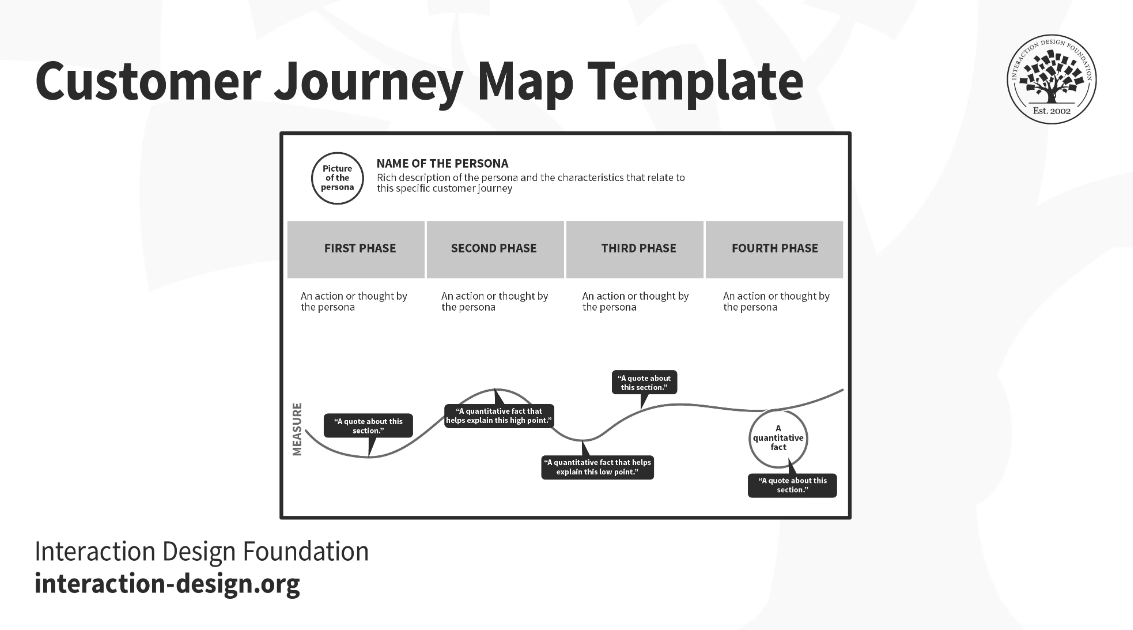
\includegraphics[width=0.70\textwidth]{Cap3/Figuras/CustomerJourneyMapEjemplo.png}
  \caption{Ejemplo de Customer Journey Map (Interaction Design Foundation, 2020b).}
  \label{fig:35}
\end{figure}

En está representación, el Customer Journey Map se divide en diferentes secciones. En la zona superior se muestran los datos generales del usuario, seguido de las etapas o también llamados puntos de contacto. En cada punto se agrega la información relacionada a los pensamientos, acciones y experiencias del usuario, los cuales están basados en la información recolectada, tal como el mapa de empatía o el diagrama de afinidad, entre otros. Finalmente se muestran los canales de cada punto de contacto, que son aquellos detalles de cómo se lleva a cabo la interacción, tal como por correo electrónico, usando un sitio web, etcétera.

Está herramienta permite una comprensión detallada de la experiencia de un usuario en cada punto de un producto, a partir de un enfoque basado en $"$un día en la vida de un usuario$"$ que genera información útil de cómo es el punto de vista de un usuario con un sistema en un ambiente cotidiano. Esto da como resultado, la oportunidad de llevar la empatía a un diseño que se adopte de mejor forma a las necesidades de un usuario, así como eliminar o evitar de forma eficiente los puntos de frustración tanto como sea posible.

%------------------------------------------------------------
%	Evaluaciones con el usuario
%------------------------------------------------------------

\section{Evaluaciones con el usuario}
\label{EvaluacionesCap3}

Las evaluaciones con el usuario consisten en una serie de pruebas, en las que se solicita al usuario realizar ciertas actividades, comisionadas por una persona denominada como evaluador. Con estas evaluaciones, el o los diseñadores pueden identificar posibles problemas que difícilmente estos podrían encontrar por la gran familiaridad y el manejo de un proyecto. Con las observaciones encontradas por los diseñadores y el evaluador, se logra identificar la descripción, procedimientos, limitaciones y problemas en el diseño.

%------------------------------------------------------------
%	Usabilidad
%------------------------------------------------------------

\subsection{Usabilidad}
\label{UsabilidadCap3}

% REFERENCIA
Hassan (2002) señala que la usabilidad es la disciplina encargada de estudiar la forma de diseñar sistemas, con el fin de brindar a los usuarios una forma fácil, cómoda e intuitiva de interactuar con un sistema, un producto o un servicio.

% REFERENCIA
El principal objetivo de la usabilidad, es lograr que el producto final sea usable para los usuarios. Hassan (2002) propone que una buena forma de lograr el objetivo, es crear un diseño del sistema centrado en el usuario. A diferencia del diseño centrado en la tecnología, que se centra el la forma más sencilla y cómoda de implementar un sistema, el diseño centrado en el usuario se enfoca en resolver las necesidades de los usuarios objetivo de forma fácil, por medio de estudios de los usuarios, creando herramientas, en las que se encuentran la técnica Persona y el Customer Journey Map, mencionados anteriormente, entre otros que puedan extraer información útil y relevante para mejorar la experiencia para el usuario.

Existe un concepto que se encuentra estrechamente relacionado a la usabilidad, denominado $"$findability$"$, que se refiere a la posibilidad de que cierta información sea encontrada o recuperada de forma accesible. La $"$findability$"$ proporciona la intervención de motores e índices de búsqueda, que facilita el proceso de recuperación o búsqueda de información. La usabilidad se apoya de diferentes conceptos para mejorar el proceso de diseño, entre ellos la $"$findability$"$, con el fin de permitir una navegación más sencilla e intuitiva dentro del ambiente de un sistema para disponer de los datos requeridos de forma sencilla.

Otro concepto del que se apoya la usabilidad, es la accesibilidad, que tiene como objetivo proveer diferentes formas de interacción para que los usuarios con alguna discapacidad puedan tener una forma de interacción para acceder a los contenidos del sistema. Así mismo, la accesibilidad propone que el contenido de un sistema debe poder proveer su contenido en diferentes tipos de dispositivos sin importar el hardware o software.

Finalmente, la usabilidad se apoya también en la utilidad, que se refiere a la cualidad de cubrir satisfactoriamente las necesidades del usuario.

% REFERENCIA
Es así como la usabilidad se convierte en la aplicación de un conjunto de conceptos para desarrollar un producto interactivo intuitivo y fácil de usar. Hassan y Ortega (2009c) mencionan algunos componentes principales que brinda la usabilidad.

\begin{itemize}
  \item \textbf{Facilidad de Aprendizaje.} Se refiere a la facilidad que muestran los usuarios para llevar a cabo las tareas para lograr sus objetivos por primera vez en el sistema.
  \item \textbf{Eficiencia.} En relación al tiempo se tardan los usuarios en realizar las tareas una vez que ya han aprendido el funcionamiento del sistema. Entre menor sea el tiempo que se tardan realizando las tareas, más eficiente es el sistema.
  \item \textbf{Cualidad de ser recordado.} Se refiere al tiempo en que los usuarios recuerdan o adquieren conocimiento del producto después de no ser usado por un periodo de tiempo. Entre menor sea el tiempo para recordar, mejor será la cualidad de ser recordado.
  \item \textbf{Eficacia.} La eficiencia se determina por los errores que comete el usuario en el sistema. Se considera la gravedad de los errores y la rapidez en la que deshacen las consecuencias de haberlos cometido. Entre menos errores se comentan y entre menor sea el tiempo de su solución, más eficiente será el sistema.
  \item \textbf{Satisfacción.} Es la decisión del usuario como resultado de su experiencia en la interacción con el sistema. Se determina lo agradable y sencillo que le pareció para lograr satisfacción al usar el sistema.
\end{itemize}

Por otro lado, es importante contar con un proceso de evaluación de usabilidad, para corroborar que la implementación cumpla con los objetivos que ofrece la usabilidad. Además, las evaluaciones son útiles para encontrar errores o comportamientos que podrían resultar confusos para los usuarios.

Existen diferentes tipos de evaluación que apoyan la valoración de usabilidad de un producto, tal como los cuestionarios, que consisten en responder una serie de preguntas bien definidas y elaboradas por expertos, o los test de usabilidad, que consisten en realizar pruebas con usuarios usando el sistema o producto y analizando su comportamiento e interacción.

%------------------------------------------------------------
%	Cuestionario de usabilidad (SUS)
%------------------------------------------------------------

\subsection{Cuestionario de usabilidad (SUS)}
\label{SUSCap3}

% REFERENCIA
Existen diferentes formas de realizar la evaluación de la usabilidad de un sistema, entre las que se encuentra la escala de usabilidad del sistema o SUS (System Usability Scale). Brooke (1995), señala que SUS es una herramienta creada por John Brooke en 2986, la cuál permite medir la usabilidad de un sistema a partir de un cuestionario con diez reactivos, cada uno de los cuales tiene cinco opciones de respuesta que van desde $"$Fuertemente de acuerdo$"$ a $"$Fuertemente desacuerdo$"$.

SUS provee una serie de beneficios y puntos a considerar durante su aplicación. Algunos de los beneficios que ofrece está herramienta son los siguientes.

\begin{itemize}
  \item Es una herramienta que permite administrar a los participantes fácilmente.
  \item Se puede aplicar a una cantidad pequeña de muestras con resultados fiables.
  \item Puede determinar fácilmente si un sistema es utilizable o inutilizable.
\end{itemize}

% REFERENCIA
Por otro lado, Brooke (1995) propone las siguientes consideraciones al usar la herramienta.

\begin{itemize}
  \item El sistema de puntuación para determinar la usabilidad del sistema puede resultar complejo.
  \item Cuando se obtiene el resultado final de usabilidad en una escala de 0 a 100, no se debe interpretar como un valor que define un porcentaje.
  \item SUS es una herramienta que permite clasificar la facilidad de uso, la aplicación o el entorno, pero no funge el rol de ser un diagnóstico del sistema.
\end{itemize}

% REFERENCIA
Anteriormente se comentó que Brooke (1995) sugiere calificar y evaluar con diez reactivos. Se proponen los siguientes reactivos, que deben ser adaptados al sistema o particularidades que son útiles para formar parte de los resultados.

\begin{enumerate}
  \item Creo que me gustaría usar este sistema con frecuencia.
  \item Encontré el sistema innecesariamente complejo.
  \item Pienso que el sistema es fácil de usar.
  \item Creo que necesitaré el apoyo de un técnico para poder utilizar este sistema.
  \item Encontré que las diversas funciones de este sistema estaban bien integradas.
  \item Pienso que había demasiada inconsistencia en este sistema.
  \item Me imagino que la mayoría de la gente aprenderá a usar este sistema muy rápidamente.
  \item Encuentro el sistema muy engorroso de usar.
  \item Me sentí muy confiado usando el sistema.
  \item Necesito aprender muchas cosas antes de poder ponerme en marcha con este sistema.
\end{enumerate}

Nótese con atención que cada reactivo está estructurado de forma que los reactivos impares (1, 3, 5, 7, 9) se refieren a enunciados con carácter positivo, mientras que los reactivos pares (2, 4, 6, 8, 10) son enunciados negativos.

Para las preguntas con carácter o actitud positiva, se toma el resultado de los usuarios en la escala de 1-5 y se le resta una unidad. En cambio, para las preguntas de carácter negativo, se le resta el resultado del usuario a un valor fijo de 5.

Una vez que todos los usuarios han respondido el cuestionario, se deben interpretar los resultados a partir de un proceso específico propuesto por SUS. El proceso de interpretación de resultados consiste en convertir las puntuaciones de los participantes en un número nuevo.

Los valores modificados anteriormente se suman para cada tipo de pregunta, se suma por cada uno de los usuarios que respondieron el cuestionario. El valor total de la suma se multiplica por 2.5. Finalmente, se obtiene el promedio de la suma del valor total de cada usuario que se obtuvo anteriormente.

El valor resultante se asocia a una puntuación definida por SUS, mostrada a continuación.

\begin{itemize}
  \item Si el valor es menor o igual a 25 puntos, entonces el sistema se considera pésimo.
  \item Si el valor se encuentra entre el rango de 26-39 puntos, entonces el sistema se considera pobre.
  \item Si el valor se encuentra entre el rango de 40-51 puntos, entonces el sistema se considera suficiente.
  \item Si el valor se encuentra entre el rango de 52-73 puntos, entonces el sistema se considera bueno.
  \item Si el valor se encuentra entre el rango de 74-85 puntos, entonces el sistema se considera excelente.
  \item Si el valor es mayor de 86 puntos, entonces el sistema se considera extremadamente bueno.
\end{itemize}

Estas escalas se muestran en la figura \ref{fig:36}.

% \begin{figure}[h]
\begin{figure}
  \centering
  \includegraphics[width=0.70\textwidth]{Cap3/Figuras/Clasificación de calificaciones de puntajes SUS.jpg}
  \caption{Clasificación de calificaciones de puntajes SUS. Brooke, J. (2013).}
  \label{fig:36}
\end{figure}

%------------------------------------------------------------
%	Proceso de evaluación del grupo ESIE
%------------------------------------------------------------

\subsection{Proceso de evaluación del grupo ESIE}
\label{ESIECap3}

El grupo ESIE ha desarrollado un proceso estándar que permite evaluar la usabilidad. Este proceso propone una serie de herramientas, pasos y participantes asignados a un rol específico que tienen un papel fundamental durante el proceso.

Las herramientas sirven como apoyo para recabar información de un proceso de evaluación. En particular, para este proyecto se utilizaron las siguientes herramientas.

\begin{itemize}
  \item \textbf{Hipótesis de la prueba.} Es un documento que toma la información de seis puntos relevantes.
  \begin{itemize}
    \item Estado de la interacción. Es el punto o estado en que se encuentra el sistema antes de realizar alguna tarea específica en el sistema.
    \item Hipótesis. Es la suposición de lo que se espera en el comportamiento del usuario al realizar una actividad específica.
    \item Tarea. Corresponde a la solicitud que se indicará al usuario para realizar cierta tarea en el sistema. Esta debe ser concreta, directa, clara y sin palabras que infieran cómo resolver la tarea.
    \item Desarrollo de la tarea. Es la acción que se debe realizar en el sistema para cumplir la tarea solicitada. Está información sólo la conoce el evaluador durante la evaluación, más no el usuario.
    \item Tiempo estimado. Es el tiempo aproximado que se estima para poder realizar la tarea.
    \item Resultado. Son las anotaciones que determinan si la tarea se resolvió satisfactoriamente, dependiendo de la hipótesis propuesta. Además se pueden incluir comentarios extra como dificultades o imprevistos al realizar la tarea.
  \end{itemize}
  Está herramienta puede dar paso a la creación del documento de actividades de la prueba.
  \item \textbf{Cuestionario de entrada.} Es un cuestionario con reactivos en los que se solicita información del usuario, tal como su edad, el tipo de herramientas y dispositivos que utiliza, así como sus interés y frecuencia con la que usa las herramientas. Estas preguntas van enfocadas a saber información que este relacionada al proyecto que se evalúa.
  \item \textbf{Protocolo de bienvenida.} Es un documento que consiste en la presentación de objetivos de la evaluación. Así mismo, se presenta el monitor y presenta las funcionalidades generales del sistema. Se pone especial detalle en expresar que la evaluación es sobre la usabilidad del sistema, más no del usuario en particular.
  \item \textbf{Actividades de la prueba.} Es un listado con todas las actividades que debe realizar el usuario. Está herramienta es un apoyo para el encargado de la evaluación.
  \item \textbf{Cuestionario de usabilidad.} Es un cuestionario que contiene reactivos específicos para determinar la usabilidad del sistema. En particular, para este proyecto se usa el cuestionario de usabilidad SUS, desarrollado en la sección \ref{SUSCap3}.
  \item \textbf{Cuestionario de percepción subjetiva.} Es un cuestionario que contiene reactivos de tipo escala, en la que se identifican particularidades de la interfaz de usuario del sistema. La escala que toman los reactivos van de uno a nueve, en donde uno corresponde a escalas no favorables y nueve a percepciones satisfactorias y positivas.
\end{itemize}

Por otra parte, el proceso de evaluación del grupo ESIE propone un conjunto de roles con tareas específicas a desarrollar durante la evaluación.

\begin{itemize}
  \item \textbf{Expertos.} Son personas encargadas del diseño de los instrumentos, mencionadas en la sección anterior, y el análisis de la información de los resultados de las pruebas.
  \item \textbf{Monitor.} Es la persona encargada de dirigir al usuario con las actividades que debe realizar como forma de guía.
  \item \textbf{Observador.} Es la persona encargada de supervisar la evaluación. Verifica que no se omita ninguna de las actividades, así como realizar un respaldo de la evaluación por medio de videos, fotografías u escritos en notas.
  \item \textbf{Anfitriones.} Son las personas encargadas de tener un control y coordinación para verificar que los usuarios respondan completamente y tener organización de los resultados de cada usuario.
\end{itemize}

El proceso de evaluación del grupo ESIE propone tres fases para realizar la evaluación de usabilidad, mismas que se mencionan a continuación:

\begin{itemize}
  \item \textbf{Primera fase.} El anfitrión o anfitriones dan la bienvenida a los usuarios y solicita que llenen los documentos de perfil de usuario, el cuál consta de información como edad, escolaridad, aplicaciones que usa, dispositivos que maneja, la frecuencia con las que se utilizan, entre otros. Es importante recalcar, que en está fase se hace la solicitud de consentimiento de los usuarios para poder registrar la evaluación por medio de videos y fotografías, con el fin de usarse como apoyo al análisis de la evaluación.
  \item \textbf{Segunda fase.} En está fase, se provee al usuario de todas las herramientas necesarias para poder manejar el sistema, dentro de un espacio sin distracciones. En este punto, el monitor toma el mando en el proceso de evaluación, el cuál estará cerca del usuario o usuarios, quienes tienen frente a ellos el dispositivo con la aplicación. Es importante localizar al monitor en un espacio que no obstruya las cámaras, micrófonos o cualquier otro dispositivo de registro.
  
  El papel del monitor consiste primeramente en leer una carta de bienvenida, la cual especifica las reglas a seguir durante la evaluación, así como los objetivos, motivos y datos extra que se esperan obtener como resultado de la evaluación. Posterior al término de la lectura de la carta de bienvenida, se crea un espacio de dudas, en la que se pregunta a los usuarios si hay algún punto que no sea claro. En caso de haber dudas, se responde a ellas, sin dar información de cómo realizar las actividades, en caso contrario, se procede al siguiente paso de está fase.
  
  El monitor comienza a leer una serie de actividades en voz alta, el cuál se conoce como guión de actividades. Las actividades deben ser completadas por los usuarios paso a paso como lo sugiere el monitor en el momento en que se sugiera. Estas actividades contienen todas las funcionalidades de una aplicación, por lo que se orienta al usuario a realizar todos las tareas que haría un usuario final.
  
  Mientras todo este proceso transcurre, el observador puede tomar notas de información que considere relevante para el análisis, tal como las reacciones al realizar alguna tarea o indagar en una funcionalidad en la aplicación. Cada vez que se termina una actividad, el monitor marca el apartado designado a está actividad como completada y procede a leer la siguiente actividad. Es importante mencionar que una actividad no se puede dar como concluida y pasar a la siguiente si no se ha completado, sin embargo, sí puede dar sugerencias de apoyo después de cierto tiempo. En cada actividad, se coloca un registro del tiempo en que el usuario tardó en realizar la tarea.
  \item \textbf{Tercera fase.} Se solicita a los usuarios que respondan los cuestionarios de usabilidad y algunos otros cuestionarios extra que se consideren oportunos para extraer información útil para el análisis, tal como un cuestionario de percepción. Estos cuestionarios pueden contener una sección de comentarios adicionales que pudieran dejar los usuarios. Finalmente se agradece a los usuarios por su participación y con ello concluye el proceso de evaluación.
\end{itemize}

% REFERENCIA
Antes de realizar las pruebas, es primordial considerar una serie de cuestiones para obtener la información más útil posible para los análisis. Entre estos puntos, se encuentra la buena selección de participantes. El reclutamiento de un participante debe asegurar que cumple un perfil acorde con los usuarios reales que usarán el sistema. Kuniavsky (2003) señala que hay tres pasos a seguir para el reclutamiento de los participantes.

\begin{itemize}
  \item Determinar la audiencia del sistema o interfaz a evaluar.
  \item Encontrar participantes que representen la audiencia a la que está dirigido el sistema.
  \item Convencer a los usuarios a participar en la prueba.
\end{itemize}

% REFERENCIA
Una vez cumplidos los tres pasos anteriores, se procede a aplicar las pruebas a todos los participantes por separado o en conjunto en caso de así requerirse. Kuniavsky (2003) propone algunos requisitos que deben cumplir las tareas encomendadas por el evaluador.

\begin{itemize}
  \item \textbf{Ser razonables.} Solicitar tareas que un usuario real realizaría en el sistema.
  \item \textbf{Estar descritas en términos de objetivos finales.} La tarea debe estar contextualizada en una motivación mayor.
  \item \textbf{Ser específicas.} La tarea debe describir objetivos concretos.
  \item \textbf{Ser factibles.} Se evalúa el diseño y usabilidad a partir de los usuarios, pero nunca se evalúa a los usuarios o su manejo sobre el sistema.
  \item \textbf{Duración razonable.} Para tareas que requieren demasiado tiempo, se recomienda descomponer la tarea en subtareas.
\end{itemize}

Así mismo, estas pruebas pretenden encontrar los puntos específicos en los que el usuario se equivoca o se detiene al realizar alguna tarea solicitada, así como tratar de entender cómo es que surgieron esos problemas a partir de la observación del participante.

Por lo general, al final de la prueba se ofrece algún tipo de recompensa como agradecimiento a la participación en las pruebas. Una vez recolectados los datos se procede a analizar los resultados, con el fin de encontrar mejoras en el diseño, siguiendo así el ciclo del diseño centrado en el usuario mostrado en la figura \ref{fig:33}.

Como se mencionó anteriormente, el diseño centrado en el usuario es un proceso iterativo, en el que cada versión de la interfaz corresponde a una iteración del proceso. Es por ello que las evaluaciones realizadas a los participantes, los resultados y la planificación de mejoras respecto a los análisis de las pruebas no reflejan la finalización del diseño de la interfaz, ya que posiblemente, esta pueda estar sujeto a nuevos cambios. Es por ello que el diseño centrado en el usuario provee un mecanismo de extensión al diseño de la interfaz.

%------------------------------------------------------------
%	Resumen
%------------------------------------------------------------

\section{Resumen}
\label{ResumenCap3}

En este capítulo se define una interfaz de usuario como un medio de interacción entre un sistema interactivo y un usuario. Se considera un conjunto de guías y principios para el diseño de la interfaz, así como algunas características provenientes de las teorías micro-HCI, que son aplicadas para la evaluación y el mejoramiento del diseño.
Posteriormente se definen las características y ventajas principales de diferentes tipos de interfaces, conocidas como interfaces multimodales o inteligentes. En particular, se pone especial énfasis en las características de las interfaces basadas en voz, tal como el procesamiento del sonido. A partir de está información, se introducen los dispositivos basados en voz, tal como Alexa, Google Home, Google Assistant, Siri, entre otros, se presentan ventajas, desventajas y usos más frecuentes en la actualidad por los usuarios.

Finalmente, se presenta de forma teórica el Diseño Centrado en el Usuario (USD) y el proceso que sigue para el diseño de interfaces de un sistema. Como complemento, se mencionan algunas herramientas útiles para el proceso de diseño, que tienen el propósito de obtener información relevante sobre las necesidades y propósitos del usuario. Se estudian herramientas como la técnica Persona y el Customer Journey Map. Con el fin de evaluar la usabilidad del sistema, se presenta el concepto de usabilidad y una forma de evaluarla en un sistema por medio del cuestionario de usabilidad SUS y el proceso de evaluación del grupo ESIE.
